\chapter{Developer documentation}
\label{ch:impl}

This essay automates Selenium tests in a cloud-native environment using a Go-based Kubernetes operator. This section contains full usage instructions for this Kubernetes operator and in-depth explanations of its features, design philosophy, and supporting technologies.

The Kubernetes operator is a tool that automates the deployment, maintenance, and scaling of Selenium tests in a Kubernetes cluster, which will be covered in this documentation. It makes it simple for DevOps teams and developers to integrate Selenium testing into production workflows, guaranteeing that their cloud-native applications are extensively tested and optimized for performance, scalability, and dependability.

This documentation will provide all the information to know to take advantage of the capabilities of this Go-based Kubernetes operator for Selenium testing, whether you are an experienced Kubernetes developer or are just getting started with cloud-native application development. Therefore, let us get in and get to exploring!

\section{Understanding the underlying technologies}

Understanding the underlying technologies that enable the Go-based Kubernetes operator for Selenium testing is crucial before we go into its specifics. The necessity of introducing these technologies and their importance in the context of developing cloud-native applications will be covered in this section.

Due to its capacity to increase the scalability, agility, and dependability of applications running in a cloud environment, cloud-native application development has grown in popularity in recent years. The use of containerization, which offers a standardized and portable mechanism to bundle and distribute programs, is at the core of this strategy.

Popular container orchestration platform Kubernetes has become the de facto standard for scalably managing containerized applications. In addition to tools for automating these procedures, it offers a complete set of primitives for deploying, scaling, and managing containerized applications.

On the other hand, the open-source testing framework Selenium enables programmers to automate web browser testing for web applications. In the context of continuous integration and continuous delivery (CI/CD) pipelines, in particular, it has evolved into a crucial tool for maintaining the quality and performance of online applications.

It is vital to integrate Selenium testing with Kubernetes to use its advantages in a cloud-native environment. The Go-based Kubernetes operator is helpful in this situation. To automate the deployment and maintenance of Selenium tests in a Kubernetes cluster, a custom controller that extends the Kubernetes API is used.

Understanding the underlying technologies is crucial for successfully operating the Go-based Kubernetes operator for Selenium testing. By doing this, DevOps teams and developers may better understand the utility of this operator and utilize it to improve their processes for creating cloud-native applications.

\subsection{Differences between Virtual Machines and Containers}

Virtual machines and containers are two standard technologies in cloud computing and application deployment. Virtual machines and containers offer isolation and virtualization, but they differ in several important ways. The distinctions between virtual machines and containers are covered in this section.

Software-based simulations of physical devices are known as virtual machines. They execute a whole operating system on top of a hypervisor, emulating the entire hardware stack, including the processor, memory, and storage. Each virtual machine has its own virtualized hardware, operating system, and isolated environment in which it operates. As a result, it is possible to run many operating systems on a single physical machine and achieve total isolation.

On the other hand, containers are a minimal type of virtualization that works at the operating system level. Multiple applications can run on the same operating system instance thanks to containers, which use the host operating system kernel and share resources with other containers. Virtual machines can be replaced by more lightweight and practical containers, which speed up the deployment and scaling of applications.

One of the key distinctions is how virtual machines and containers use their resources. Resource wastage can occur because virtual machines need many resources to replicate a whole hardware stack. Contrarily, containers use resources better because they share the host operating system kernel.

\begin{figure}[H]
	\centering
	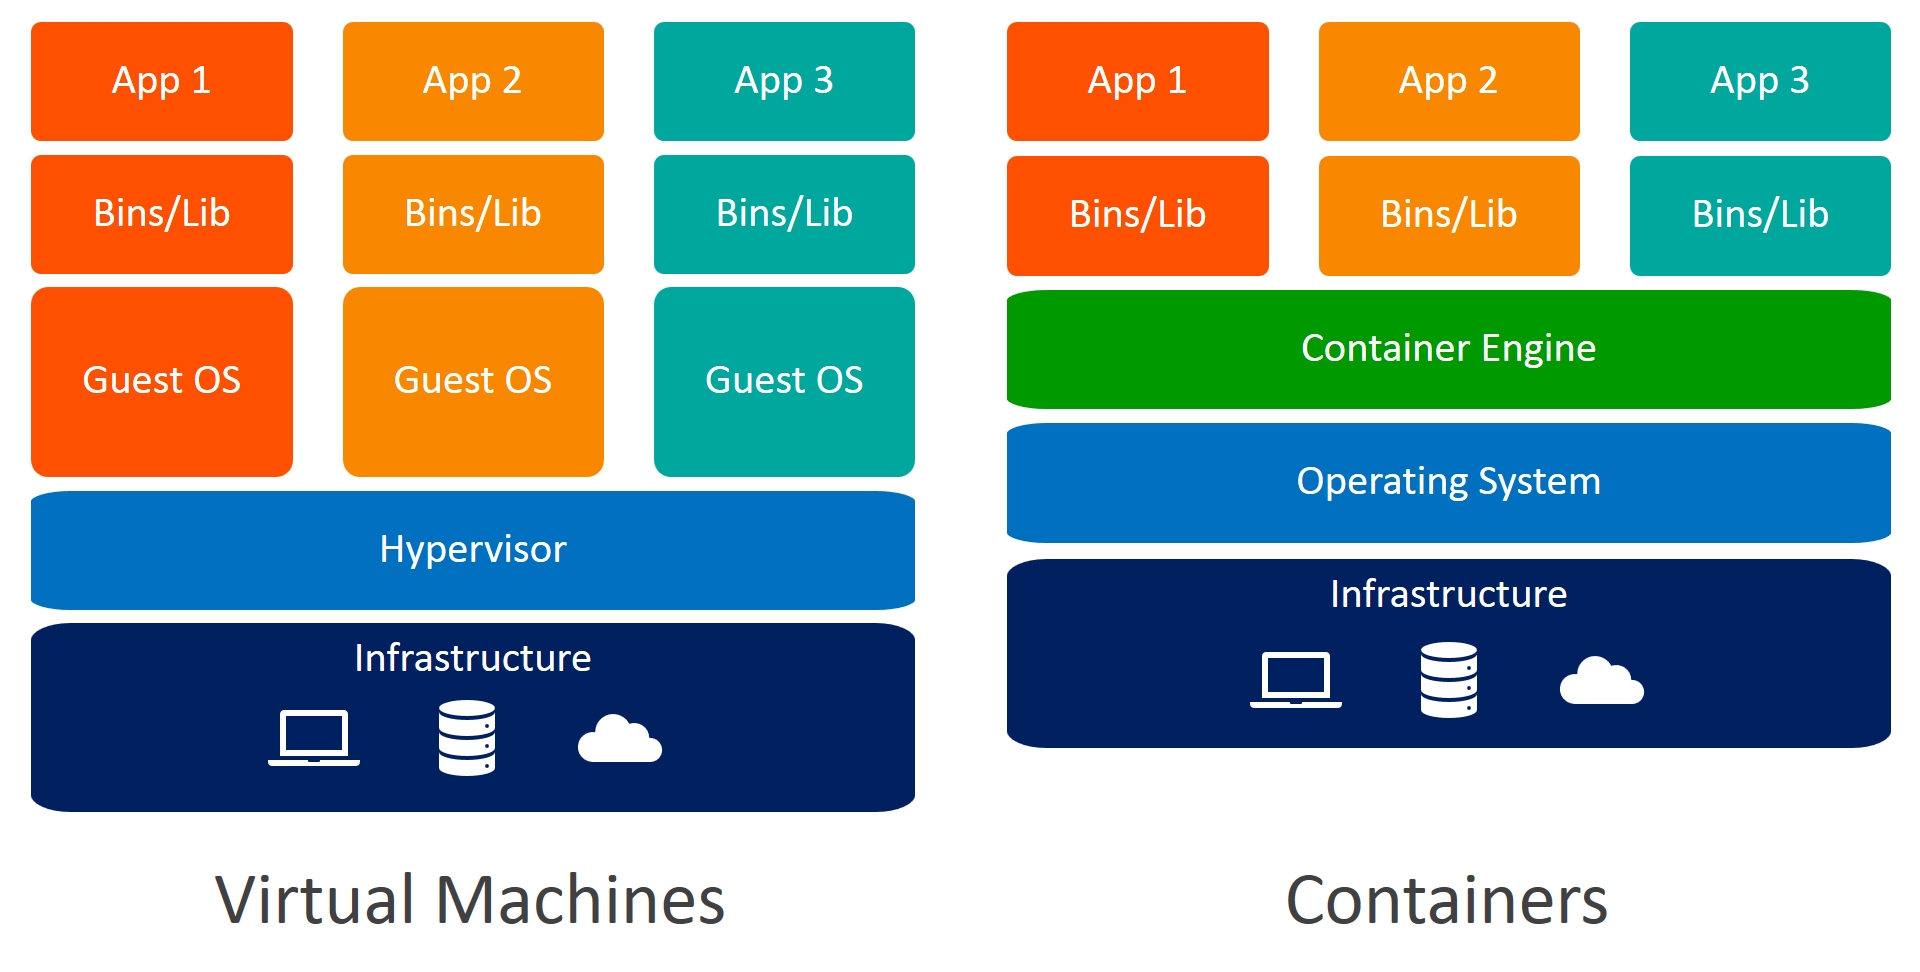
\includegraphics[width=1\textwidth]{containers-vs-virtual-machines}
	\label{fig:container-vs-vm}
\end{figure}

The starting times of virtual machines and containers are another distinction. Virtual machines typically take longer to start up because a complete operating system must be booted. In contrast, containers start up relatively instantaneously because just the containerized program needs to be started.

In conclusion, although virtual machines and containers offer virtualization and isolation, they differ in resource usage, startup time, and security, with containers providing a more portable and practical option for running applications.

\subsection{The Advantages of Container Orchestration with Kubernetes}

\begin{wrapfigure}{r}{0.25\textwidth}
    \begin{center}
        
\includegraphics[width=0.23\textwidth]{kubernetes-text}
	  \label{fig:kubernetes-logo}
    \end{center}
\end{wrapfigure}
Automating the deployment, scaling, and maintenance of containerized applications is known as container orchestration. In the age of cloud computing, container orchestration has become an essential tool for managing massive applications. The most well-known and commonly used container orchestration platform is Kubernetes.

The ability to automatically deploy and scale containerized apps is one of the critical benefits of Kubernetes-based container orchestration. Developers can declare the intended state of their application using Kubernetes' declarative configuration technique, and Kubernetes will take care of the rest. By doing this, the application can scale up or down as necessary and will continuously operate as intended.

Additionally, a variety of built-in features and extensions provided by Kubernetes enable sophisticated container orchestration capabilities. These include, among other things, automatic failover, load balancing, advanced scheduling, and service discovery. Kubernetes also offers a powerful command-line interface and API for communicating with and administering containerized applications.

Kubernetes' capacity to function on any cloud infrastructure or on-premises data center is a substantial additional benefit. No matter where containerized applications are running, Kubernetes abstracts away the underlying infrastructure and offers a standard application deployment and management method. Because of this, fully cloud-native apps that can be deployed anywhere may be created.

Additionally, Kubernetes has a sizable and vibrant open-source community, which means it is continuously developing and getting better. The community updates Kubernetes with additional functions, bug fixes, and security patches, transforming it into a dependable and safe environment for running mission-critical applications.

In conclusion, Kubernetes container orchestration is necessary for managing modern cloud-native applications. It is the best platform for managing containerized applications due to its powerful orchestration features, automation of deployment and scaling, and flexibility to run on any infrastructure. Thanks to its vibrant and expanding community, it will continue to be a safe and dependable platform for managing apps for many years.


\subsection{Fundamental Kubernetes Objects}

The open-source container orchestration platform Kubernetes automates containerized applications' deployment, scaling, and maintenance. Kubernetes enables developers to construct and manage containerized applications at scale regardless of the underlying infrastructure.

\begin{wrapfigure}{L}{0.09\textwidth}
        \includesvg[width=00.085\textwidth]{pod}
	  \label{fig:pod}
\end{wrapfigure}

A pod, a single instance of a container running on a node, is the smallest deployment unit in Kubernetes. One or more containers may be included in pods, which share the same network namespace and storage. By guaranteeing that a certain number of replicas, or exact duplicates of the pod, are active at all times, replicasets control the scaling of pods.


\begin{wrapfigure}{L}{0.09\textwidth}
        \includesvg[width=0.085\textwidth]{deploy}
	  \label{fig:deploy}
\end{wrapfigure}

A set of replicasets and pods may be managed in the desired state declaratively using deployments. By establishing a deployment and describing the number of copies and the containers' desired state, developers can ensure the application is functioning as planned. Rolling updates, rollbacks, and version control are additional features of deployments.


\begin{wrapfigure}{L}{0.09\textwidth}
        \includesvg[width=0.085\textwidth]{svc}
	  \label{fig:svc}
\end{wrapfigure}

By providing a consistent IP address and DNS name for accessing a group of replicas, services isolate network access to pods and replicasets. Services can expose pods openly to the internet or internally to other pods in the same namespace.

\begin{wrapfigure}{L}{0.09\textwidth}
    \begin{center}
            \includesvg[width=0.085\textwidth]{ns}
    	  \label{fig:ns}
      \end{center}
    \begin{center}
        \includesvg[width=0.085\textwidth]{cm}
	  \label{fig:cm}
  \end{center}
   \begin{center}
        \includesvg[width=0.085\textwidth]{cronjob}
	  \label{fig:cronjob}
  \end{center}
\end{wrapfigure}

Objects in a Kubernetes cluster are grouped using namespaces. They give a mechanism to group and protect resources, so one can use them to separate teams or applications into logical partitions inside a cluster.

Configmaps hold configuration information that running containers can access. They offer a practical method for handling application configuration information, including environment variables or configuration files.

Jobs are Kubernetes objects that execute a specified task, such as a batch job or a script, until it is finished. CronJobs, on the other hand, are objects that execute a specific operation at a predetermined time, such as executing a backup script every day at midnight.

These Kubernetes components offer a robust and adaptable infrastructure for managing containerized applications. Kubernetes allows developers to concentrate on developing code and providing business value rather than worrying about the underlying infrastructure by utilizing these abstractions and automating typical tasks.


\subsection{Kubernetes custom resources and operators}

Developers can control many facets of their application deployments using the wide range of built-in resources that Kubernetes offers. However, some applications need specialized resources that Kubernetes does not ship with. Kubernetes provides custom resources, enabling programmers to create API objects representing unique resource types.

Because they can be used to represent any resource that is not already included in Kubernetes, custom resources are crucial. These unique resources can be used to specify certain actions, like configuring a firewall just for an application or creating a unique scaling policy. Custom resources can be generated, maintained, and watched over in the same ways as built-in resources.

Making a unique resource is simply the first action in any case. Developers frequently need bespoke controllers in order to manage customized resources efficiently. A Kubernetes operator known as a controller tracks changes to a custom resource and initiates the necessary responses. The operator carries out a variety of duties, like changing a configuration, starting a deployment, or keeping track of a resource.

An efficient technique to automate complicated activities involving bespoke resources is with Kubernetes operators. Developers can design operators to give particular behavior for a unique resource. As a result, operators automate resource management rather than managing resources by hand, lowering the possibility of human error and speeding up the process.

The ability for developers to customize Kubernetes to meet their unique needs is one of the advantages of its bespoke resources and operators. Instead of constraining their workflows to fit into Kubernetes' existing architecture, developers can design new resources and operators to automate their unique workflows.

To sum up, Kubernetes' custom resources and operators are robust tools that give developers the ability to increase the functionality of Kubernetes to match their particular needs. Developers can define their API objects for custom types of resources using custom resources, and operators can automate complex activities involving these resources. Developers can create a more robust and automated Kubernetes environment that suits their unique requirements by employing custom resources and operators.


\subsection{Understanding Kubernetes Role-Based Access Control (RBAC)}

An essential security component of Kubernetes is role-based access control (RBAC), which enables users to specify explicit permissions and access policies for managing Kubernetes resources. Kubernetes administrators can control who has access to and can alter resources at a precise level with RBAC.

By establishing roles and bindings, RBAC enables Kubernetes cluster managers to manage access to the cluster. A binding ties a role to a user, group, or service account, whereas a role defines a set of rules that specify the actions a user or group can do on Kubernetes resources. Kubernetes administrators can build bespoke access policies that perfectly meet their security needs by combining roles and bindings.

Cluster roles, cluster role bindings, roles, and roles bindings are only a few of the roles and bindings the RBAC feature in Kubernetes provides. While roles and role bindings define permissions for resources inside a namespace, cluster roles, and cluster role bindings define permissions for resources across the entire cluster.

The definition of cluster-wide permissions that can be granted to individuals or groups uses cluster roles and cluster role bindings. Cluster roles are created by providing a set of rules that specify the operations that can be carried out on a resource. A user, group, or service account is bound to a cluster role by a cluster role binding. The resources indicated in the cluster role can now be accessed and modified by the user or group.

Namespace-level permissions are defined using roles and role bindings and can be given to individuals or groups. Roles are built by specifying a set of rules that limit what can be done to resources within a given namespace. By associating a role with a user, group, or service account, those accounts can access and modify resources in the namespace designated by the role.

Granular control over who can access and alter resources within a Kubernetes cluster is possible thanks to Kubernetes RBAC. RBAC allows cluster administrators to handle rights at a highly granular level, which is crucial for big businesses with detailed security requirements.


\subsection{Microservice Architecture and Kubernetes: A Perfect Match for Scalability and Agility}

Creating an application as a collection of loosely connected, independently deployable services is known as microservice architecture. Typically, each microservice only handles one task and interacts with other microservices using clear APIs.

The popularity of the microservice architecture can be attributed to a number of factors. The ability for teams to build, test, and deploy separate services independently is one of its key benefits. These can lead to shorter development cycles and more agility. Additionally, because microservices can be scaled horizontally, more service instances can be added to meet growing demand, improving the performance and scalability of the entire application.

Because it offers many features that make it simple for teams to deploy, manage, and scale microservices, Kubernetes, as a container orchestration platform, is a good fit for the microservice architecture. By enabling teams to deploy microservices as containers, Kubernetes offers a dependable and adaptable environment that can run on any infrastructure. Additionally, Kubernetes has functions like load balancing, service discovery, and automatic scaling essential for managing large-scale microservices applications.

In conclusion, microservice architecture is favored because it improves software development's flexibility, scalability, and agility. Microservices may be quickly launched, managed, and scaled to meet the demands of modern applications when used in conjunction with Kubernetes. Microservices and Kubernetes working together can speed up application development cycles, enhance application performance, and boost resilience and fault tolerance.


\subsection{Challenges of Testing Microservices and How Selenium Helps}

Although the flexibility and scalability of the microservice architecture are two of its many advantages, it also presents some unique testing challenges. Due to their distributed nature, the complexity of the system, and the requirement to ensure that all services function together without interruption, testing microservices thoroughly can be challenging. Fortunately, there are tools like Selenium that can assist in overcoming some of these obstacles.

The fact that processes are spread across several services makes it difficult to test individual services, which is one of the critical challenges with testing microservices. Additionally, it can be challenging to guarantee that each service functions correctly because adjustments to one service may impact how another behaves. Furthermore, microservices frequently use external APIs, which makes testing more challenging.

The system's intricacy poses another difficulty. It can be challenging to keep track of what is happening and where problems occur when numerous small services are communicating. This complexity can cause delays in problem resolution by making it challenging to pinpoint the source of a problem.

An open-source automated testing tool called Selenium can assist in overcoming some of these difficulties. In order to make testing web applications that use microservices simpler, it offers a set of tools for automating web browsers. Testers can mimic user interactions with a web application using Selenium to ensure all services operate as intended.

Selenium can test an application more completely and faster than manual testing since it can automate testing. Additionally, it is capable of running tests concurrently, enabling quicker feedback and shorter testing cycles. Selenium also offers an interface with other testing frameworks and tools, such as JUnit and TestNG, which makes it simpler to incorporate into already-in-place testing procedures.

In conclusion, thorough testing might be difficult because of the dispersed nature and complexity of microservices. However, by automating testing and offering a suite of tools for testing web applications that rely on microservices, tools like Selenium can help to overcome some of these difficulties. Using Selenium, testers can check that microservices interact adequately and quickly spot problems, resulting in quicker feedback and shorter testing cycles.


\subsection{An Overview of Selenium: Application Testing Tool}

Selenium is a web application testing tool. It automates testing online applications by imitating user behaviors, including button clicks, text entries, and page navigation. Developers can use Selenium to create scripts that automate time-consuming testing processes, saving time and effort compared to manual testing.

Java, Python, C\#, Ruby, and JavaScript are just a few programming languages supported by the open-source Selenium tool. Selenium WebDriver, Selenium Grid, and Selenium IDE are some of its various parts.

A programming interface called Selenium WebDriver enables programmers to automate interactions with web browsers. It offers a selection of techniques for manipulating online components like buttons, text boxes, and drop-down menus, moving between pages, and utilizing browser capabilities like tabs and windows.

Selenium Grid is a tool for simultaneously executing tests on several operating systems and browsers. It permits parallel testing, which can drastically cut down on the amount of time needed for testing.

The browser extension Selenium IDE offers a user-friendly interface for building and running Selenium tests. It enables developers to capture user interactions and produce test scripts without creating any code.

Selenium IDE stores test cases in files with .side extensions. They are JSON files that contain information about the test case, such as the name, description, and steps. The steps in a .side file describe the actions that Selenium should perform during the test, such as clicking a button or entering text into a text box.

As a result of imitating user activities, Selenium is a popular testing tool for web applications that automates the testing process. Selenium WebDriver, Selenium Grid, and Selenium IDE are some of its various parts. In order to store test cases, Selenium IDE uses .side files. It also offers a user-friendly interface for developing and running Selenium tests.


\subsection{Prometheus, Alerting and Service Monitors}

Popular open-source monitoring software Prometheus gathers, stores, and queries metrics from various sources. It offers a versatile query language and a potent data model that allow users to learn essential things about the functionality and state of their systems. However, more than simply gathering and storing metrics is required; (human) operators must also be informed when specific situations call for their attention. Prometheus alerting and service monitors are helpful in this situation.

Users can create alerting rules in Prometheus that send notifications when specific metrics exceed predetermined thresholds. Users can select from a wide variety of notification channels, including email, Slack, and PagerDuty, to name a few, and these rules can be highly configurable. Additionally, users can use Prometheus' robust query language to develop more intricate alerting scenarios.

On the other hand, service monitors are Kubernetes resources that specify how Prometheus should monitor a particular service. They enable administrators to automatically find services operating in a Kubernetes cluster and set up Prometheus to monitor those services. Service monitors specify which metrics should be collected and how they should be collected. They can also include labels to help organize the data that has been gathered.

Alerting and service monitors work together to give operators the ability to create effective monitoring and alerting systems that can identify problems before they become critical and warn the necessary parties for a quick resolution.


\section{The Operator: from Architecture to fine details}

This section discusses the architecture of the thesis project operator, providing all the information necessary to fully comprehend how its many components relate to one another and how their interdependencies operate.

In a nutshell, the operator accepts the SeleniunTest kind of custom resource, specifying the name, scheduling, browser runner service, and config map holding the selenium .side test file. As a result, the operator constructs a cronjob with the necessary permissions, which arranges the tests to run on the browser runner service when executed at the specified times. The test results are subsequently written into a SeleniumTestResult type of CR. The operator responds with its reconciliation logic, which exposes the test results in Prometheus format in a central location for Prometheus-like monitoring solutions to integrate into their alerting chain. Each component will be more thoroughly explained in this section.

In addition, viable other integration methods will be highlighted, demonstrating how adaptably a company can integrate it into its environment without resorting to quirky workarounds or modifying the operator.

\begin{figure}[H]
	\centering
	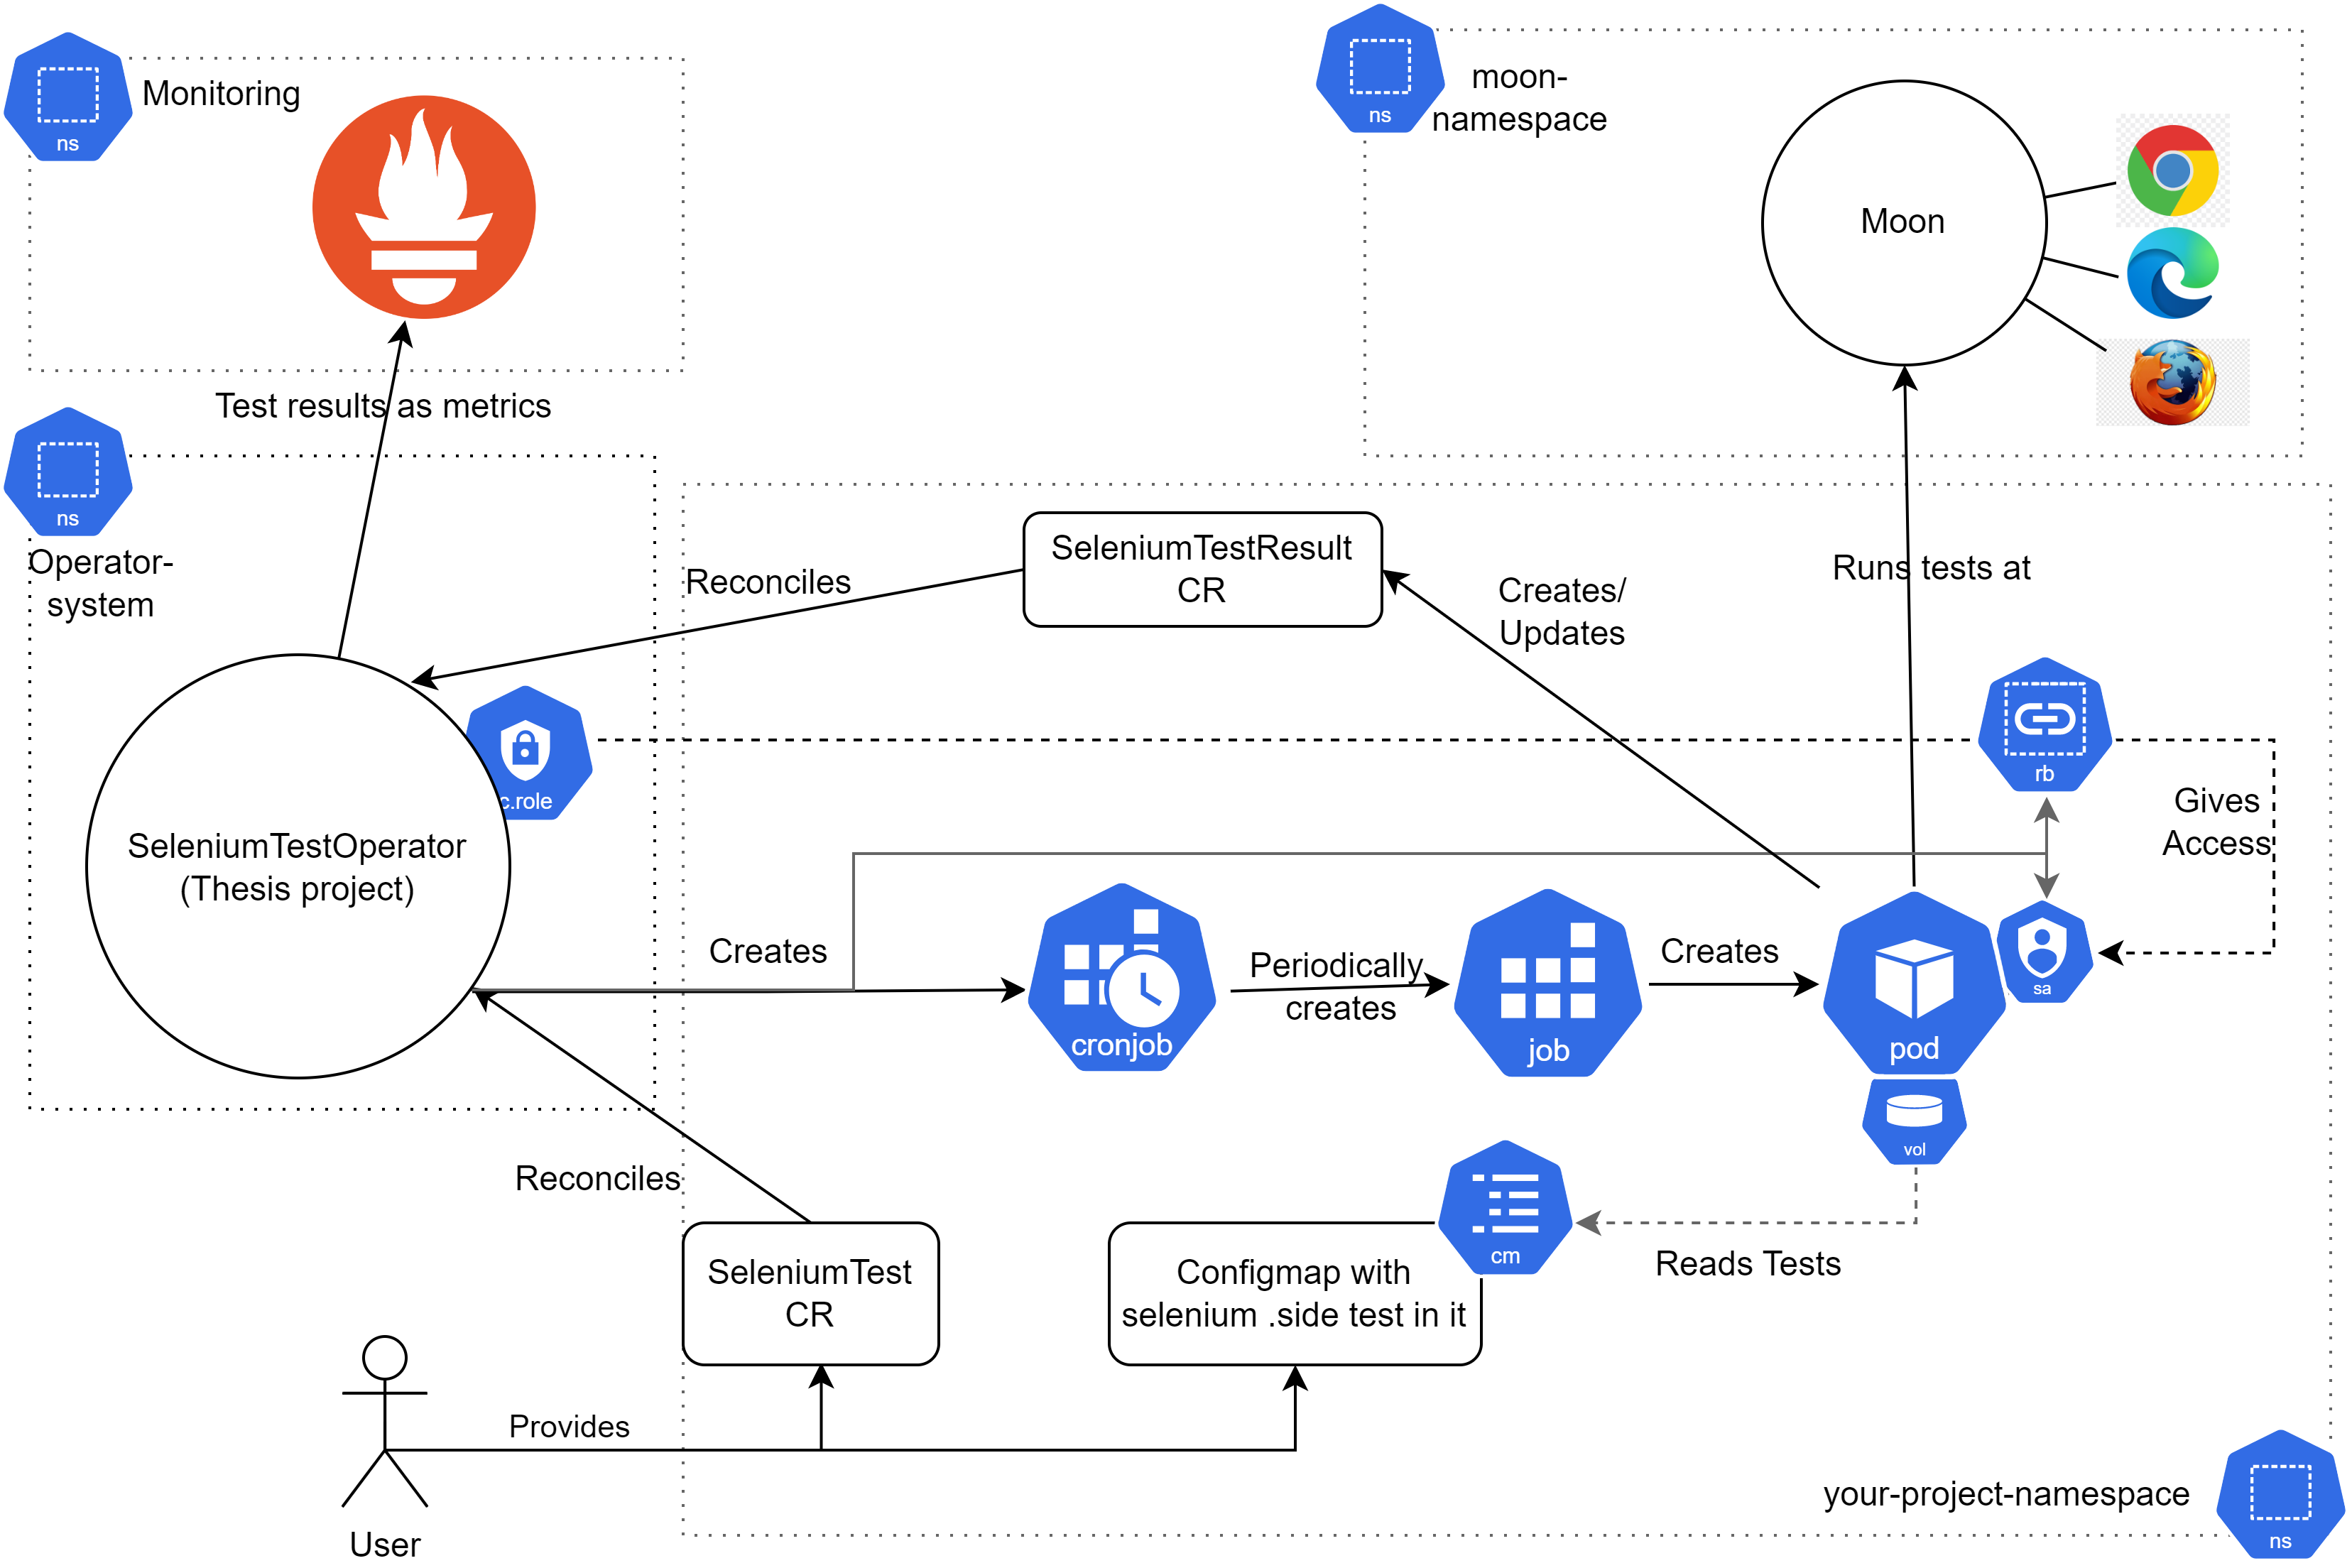
\includegraphics[width=1\textwidth]{Architecture}
	\label{fig:architecture}
\end{figure}

\subsection{User-facing components of the SeleniumTestOperator}
As shown in the user manual, the user needs a test created by the Selenium IDE exported to a .side file, and placed into a config map, to set up a test in the cluster. Additionally, the user must supply a SeleniumTest custom resource containing the necessary data about it. With the operator's deployment, a unique resource definition was also deployed for Kubernetes to comprehend these CRs.

By defining custom resources not included in the basic Kubernetes API, Kubernetes Custom Resource Definitions (CRDs) are used to expand the Kubernetes API. Developers can manage essential resources like pods, services, and deployments in the same way that they manage custom resources, thanks to CRDs.

Making a YAML file that details the custom resource's schema is part of defining a CRD. The schema specifies the attributes that can be set and the resource's structure. Additionally, it contains validation rules that guarantee the accuracy of the data entered for the custom resource.

Typically, the CRD YAML file contains the following data:

\begin{itemize}
	\item Group and version information: Indicates which API group and version the CRD is a part of. In API requests, the CRD is identified by the group and version.
	\item Kind information: gives specifics about the type of the custom resource. In Kubernetes API queries, the kind is used to specify the kind of the custom resource.
	\item Metadata: includes details on the CRD, including its name, labels, and annotations.
	\item Spec: Specifies the fields that can be set and their types, as well as the structure for the custom resource. Additionally, it includes validation rules that guarantee accurate data entry for the custom resource.
\end{itemize}

Each CRD has a corresponding go object defined within the operator, as well as a reconcile function:

\begin{lstlisting}[language={Go}]
	// SeleniumTestSpec defines the desired state of SeleniumTest
	type SeleniumTestSpec struct {
		Repository    string `json:"repository"`
		Image         string `json:"image"`
		Tag           string `json:"tag"`
		Schedule      string `json:"schedule"`
		ConfigMapName string `json:"configMapName"`
		Retries       string `json:"retries"`
		SeleniumGrid  string `json:"seleniumGrid"`
	}
	// SeleniumTestStatus defines the observed state of SeleniumTest
	type SeleniumTestStatus struct {
		CronJobName string `json:"cronJobName"`
	}
	// SeleniumTest is the Schema for the seleniumtests API
	type SeleniumTest struct {
		metav1.TypeMeta   `json:",inline"`
		metav1.ObjectMeta `json:"metadata,omitempty"`
	
		Spec   SeleniumTestSpec   `json:"spec,omitempty"`
		Status SeleniumTestStatus `json:"status,omitempty"`
	}
\end{lstlisting}

The reconcile function is the core function responsible for maintaining the desired state of a resource. The reconcile function checks to see if the resource's current state corresponds to the ideal state stated in the resource's Kubernetes manifest.

The Kubernetes API server tells the operator when a change is found in the resource, and the operator then initiates the reconcile function. The reconcile function compares the resource's present state to the desired state listed in the manifest by reading its current state. The reconcile function takes the necessary steps to resolve discrepancies between the desired and current conditions.

The reconcile function, in general, is a crucial part of a Kubernetes operator and, when appropriately used, guarantees that the resources are always kept in the desired state.

\begin{figure}[H]
	\centering
	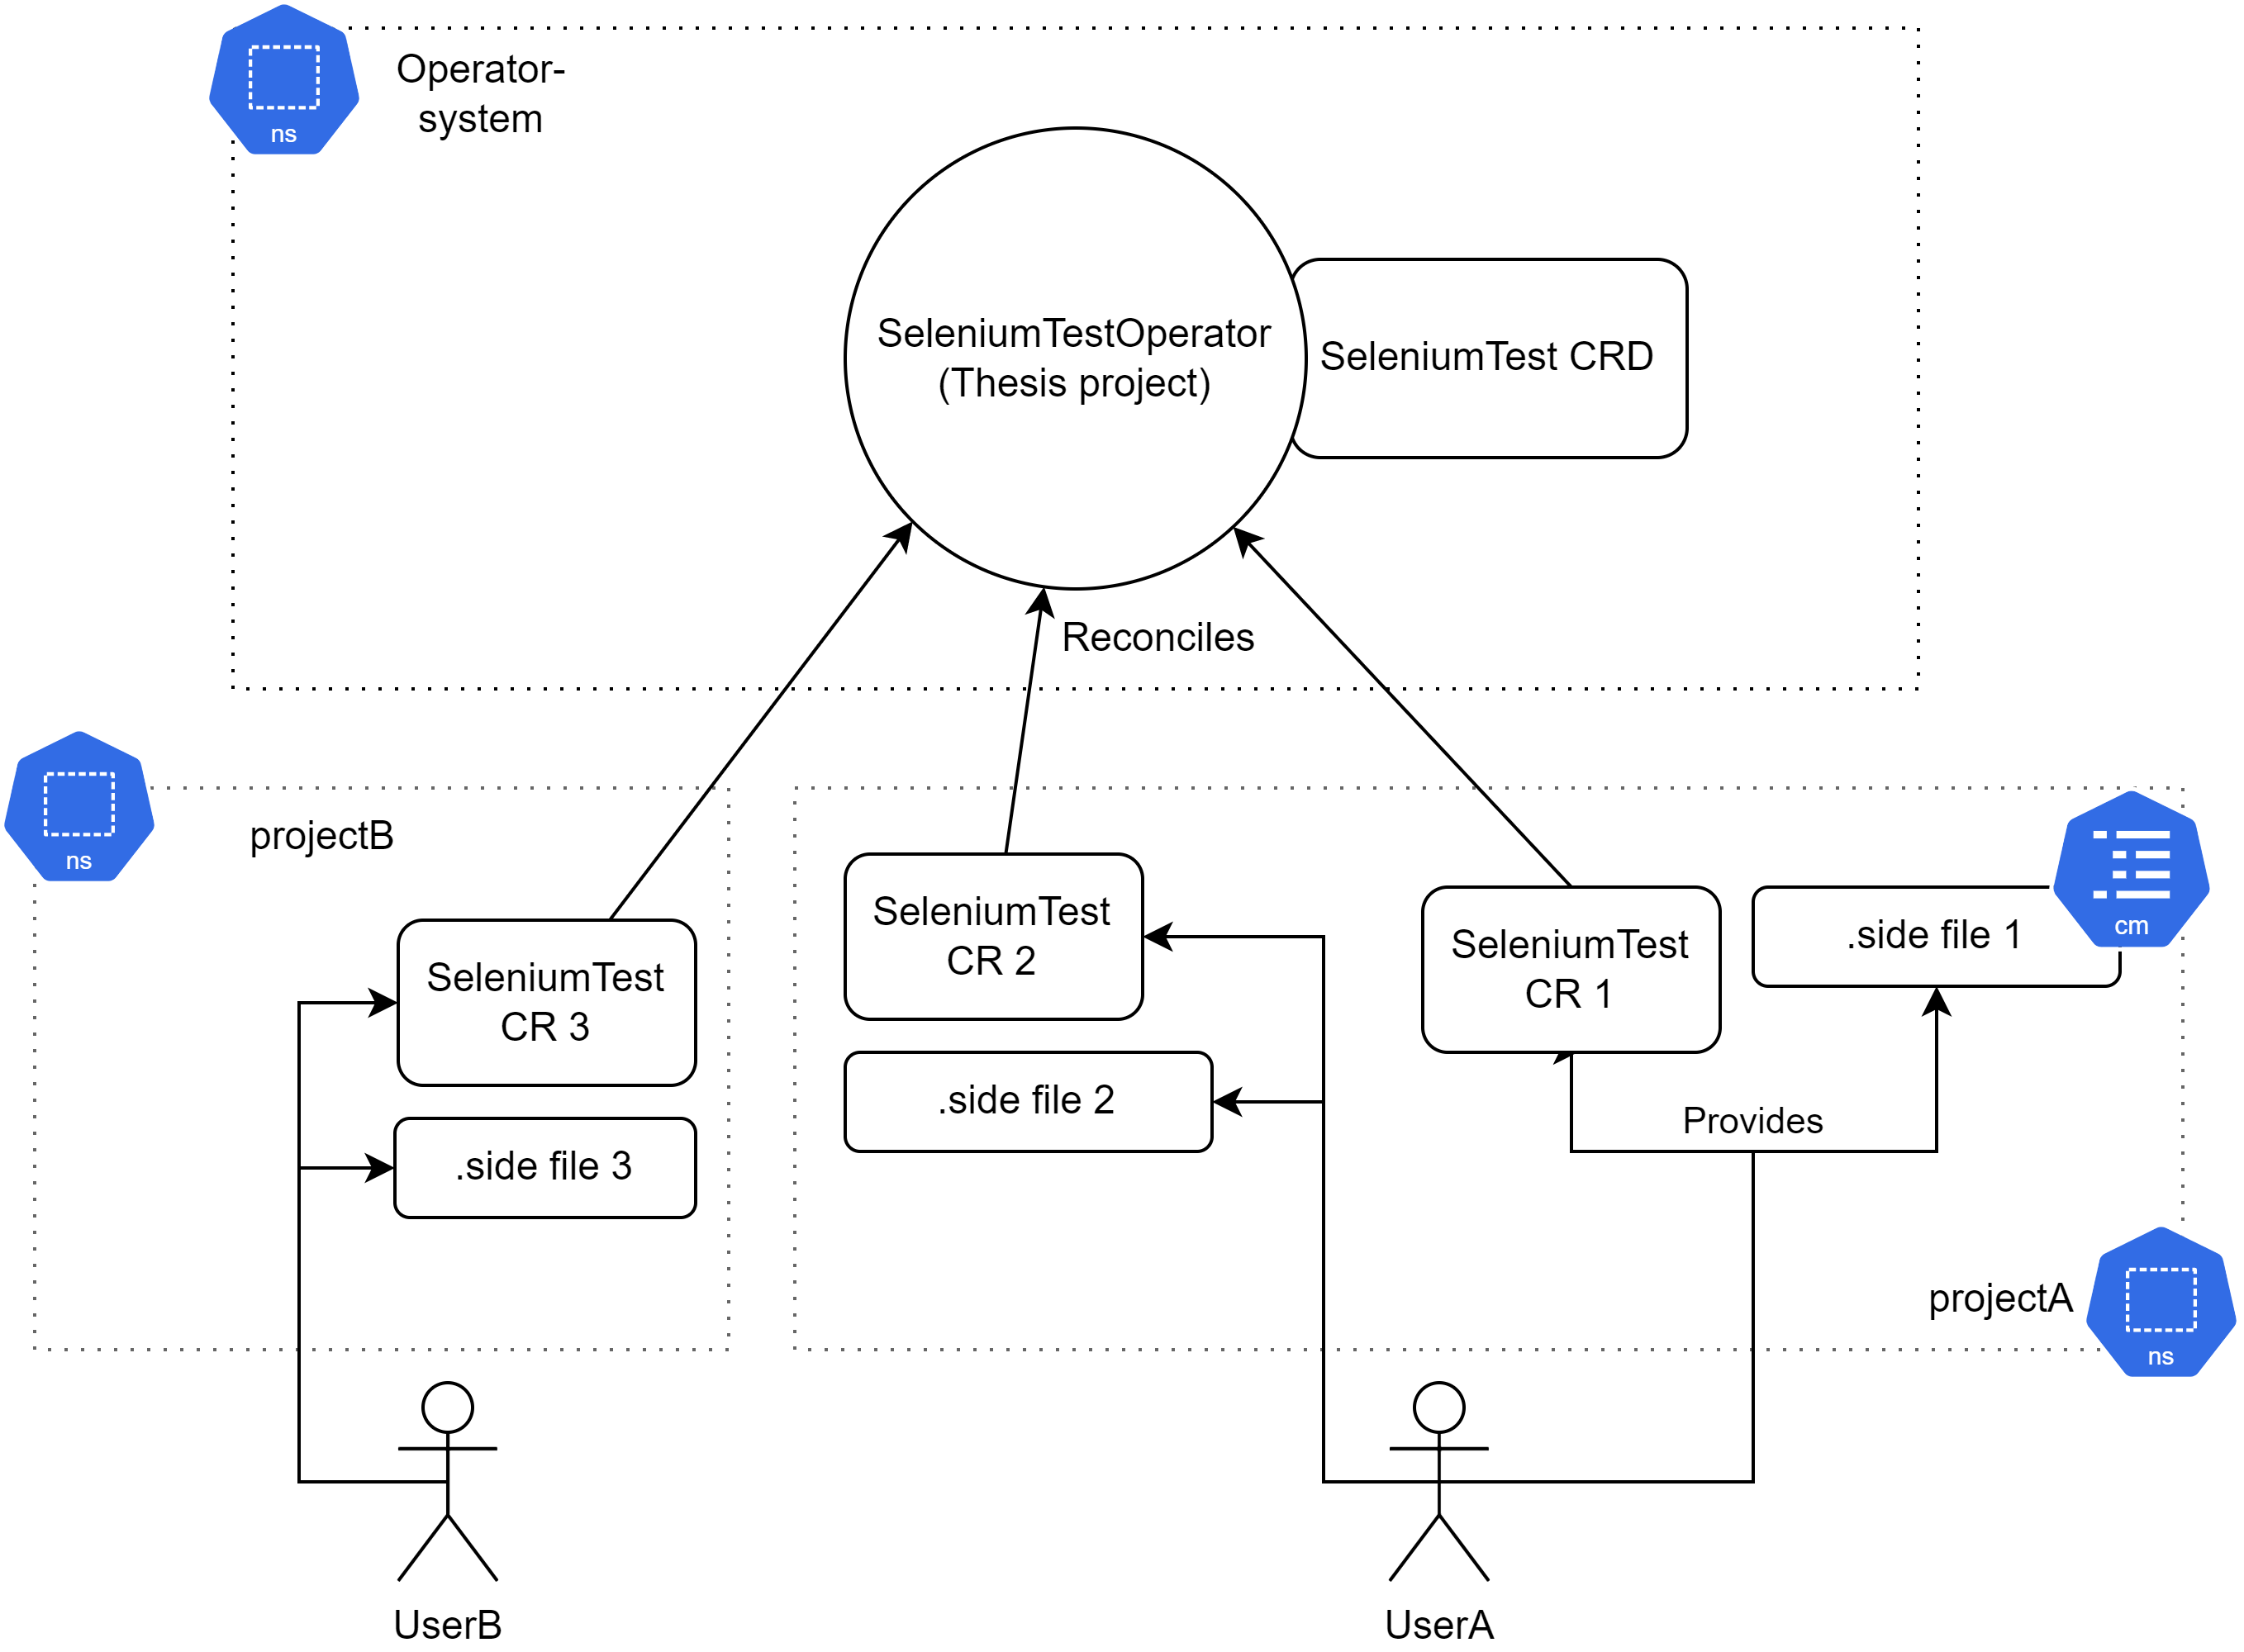
\includegraphics[width=1\textwidth]{input_arch}
	\label{fig:input_arch}
\end{figure}

\subsection{Automated scheduling of the tests}

The operator assigns all workloads to the same namespace where the user provided the CR and the configmap containing the test file to enable comprehensive monitoring between projects. This workload comprises numerous Selenium side runs wrapped in JavaScript code inside a Node.js container. Kubernetes' built-in automation is used for easier maintenance, and the workload is abstracted within pods within jobs within cronjobs.

In order to make sure that a job is consistently created at the appropriate time, the operator creates a cronjob with the specified schedule. The hash code is put after the name of the jobs, which run under the same name as the cronjob.

The test file is accessible within the containers at the "/mnt/config" folder since the operator attached the given configmap as a volume to the job's pod.

\begin{figure}[H]
	\centering
	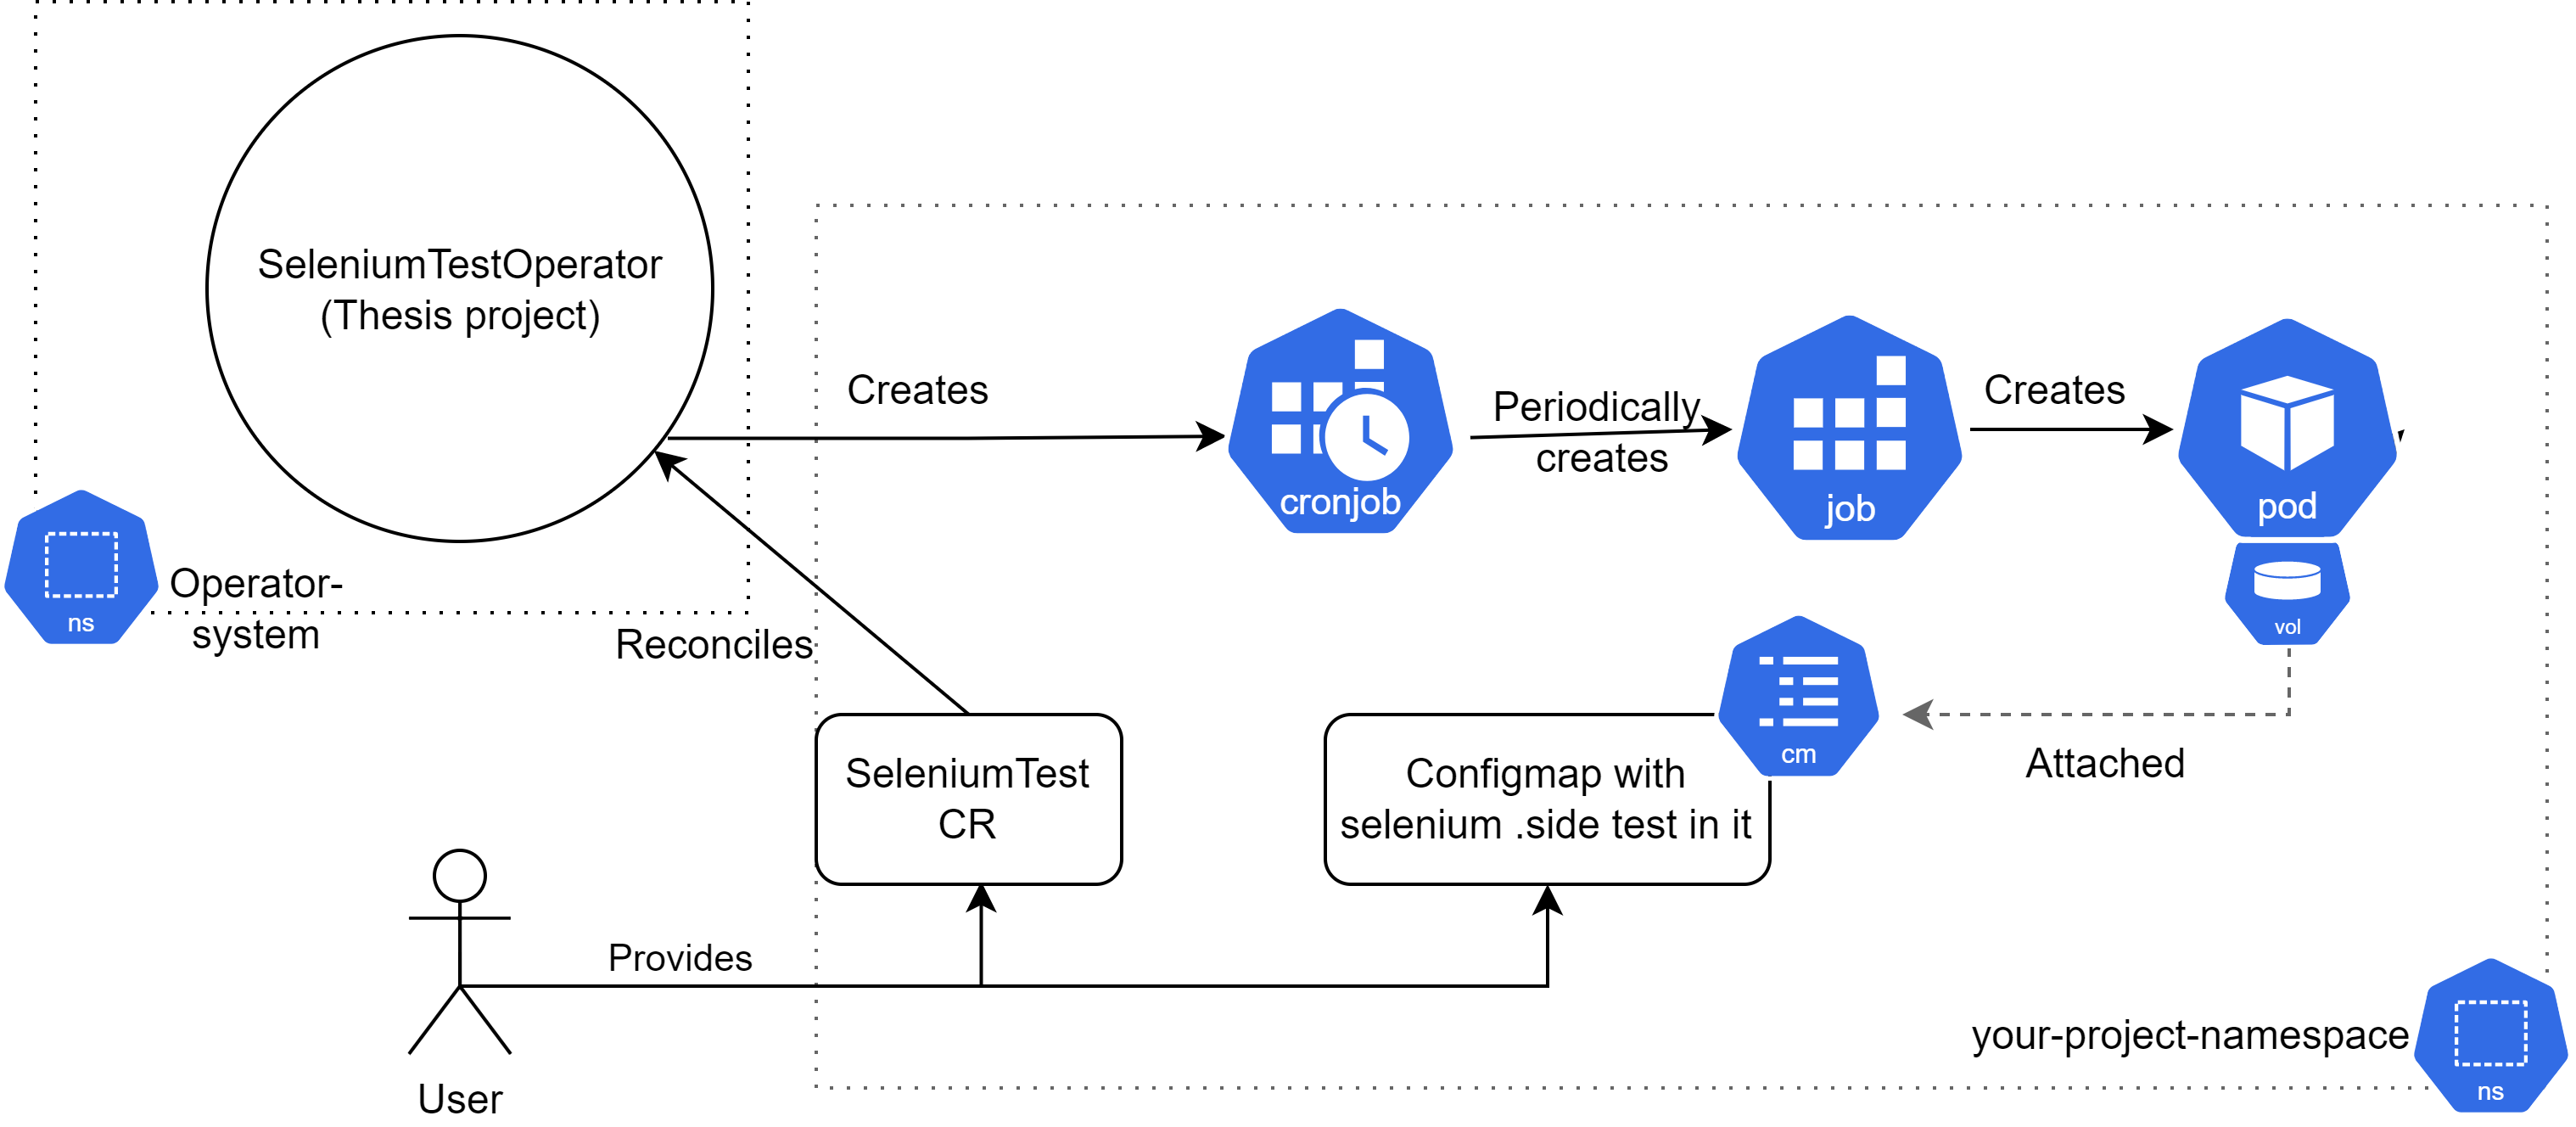
\includegraphics[width=1\textwidth]{cronjob_automation}
	\label{fig:cronjob_automation}
\end{figure}

Without explicitly stating differently, pods use the default service account, severely limiting their capacity to communicate with the cluster. Therefore, the operator has a cluster role with all the permissions the pod's script requires. The operator generates a dedicated service account in the workload namespace for each test and a role binding that links the newly established service account to the previously described cluster role.

\begin{figure}[H]
	\centering
	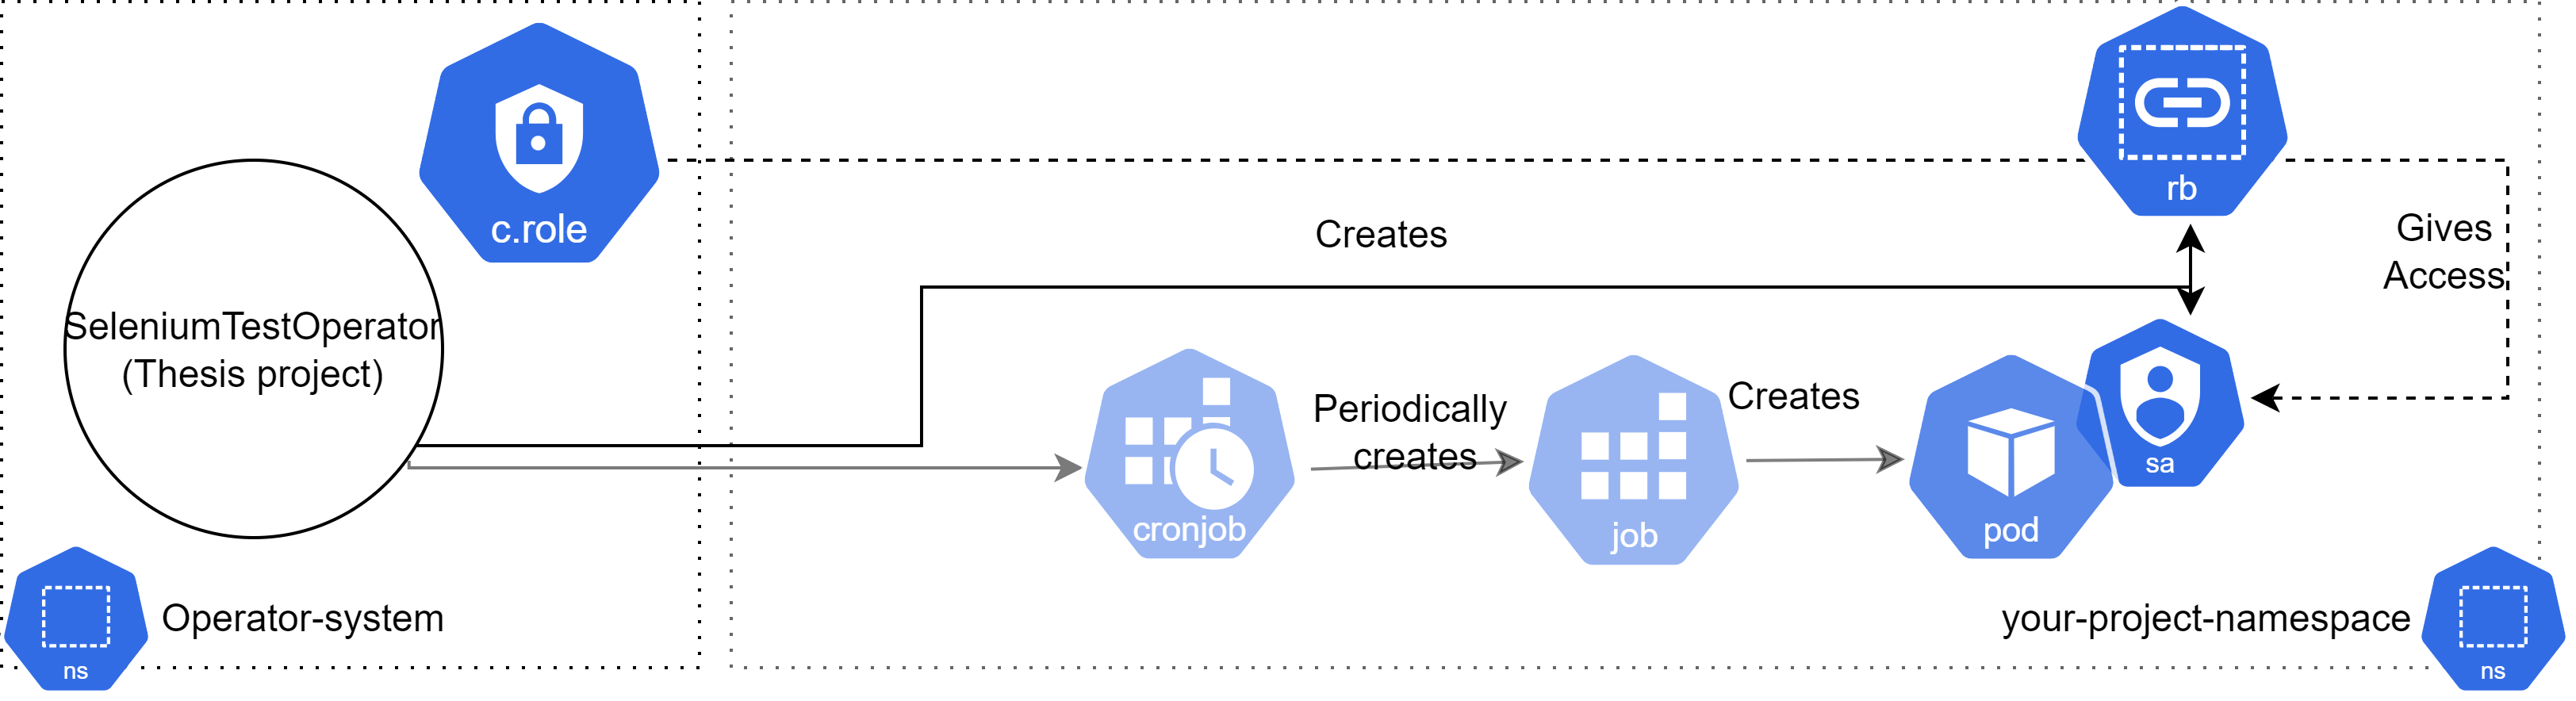
\includegraphics[width=1\textwidth]{rbac}
	\label{fig:rbac}
\end{figure}

The SeleniumTest controller's reconcile method, which has the following syntax (logging, exception handling, comments, etc., are not included here for readability in the documentation), handles the construction or validates the existence of all the objects:

\begin{lstlisting}[language={Go}]
	func (r *SeleniumTestReconciler) Reconcile(ctx context.Context, req ctrl.Request) (ctrl.Result, error) {
		instance := &seleniumv1.SeleniumTest{}

		// Validates the ConfigMap with the given name is present
		err = r.ensureConfigMap(instance)
		// Checks the ServiceAccount is present, if not, creates it
		err = r.ensureServiceAccount(instance)
		// Checks the RoleBinding is present, if not, creates it to connect the service account to the cluster role
		err = r.ensureRoleBinding(instance)
		// Ensure the CronJob is present, if not, creates it with the configmap attached as volume, with the serviceaccount above 
		err = r.ensureCronJob(instance)

		return ctrl.Result{}, nil
	}	
\end{lstlisting}

\subsection{Using Selenium WebDriver for Browser Interactions}

Interactions with web browsers are possible using the Selenium WebDriver tool. It offers a collection of procedures and instructions that mimic user operations, including clicking buttons, inputting text, and moving between pages.

A Node.js container is established with the required Selenium libraries and drivers to use Selenium WebDriver with Node.js with a Selenium Hub deployment (Moon is given as an example in this tutorial, but there are many more possibilities). The container also includes all additional dependencies needed for the tests.

The Selenium WebDriver is used within the container to communicate with the Moon. This entails creating a fresh instance of the appropriate browser, which would then be used to navigate to the desired URL and carry out any necessary interactions described with the .side test files.

Data regarding the test, including page load times, failures, and other performance indicators, is generated while the script runs. Then the test findings are processed and reported to the operator via a custom resource called SeleniumTestResult.

\begin{figure}[H]
	\centering
	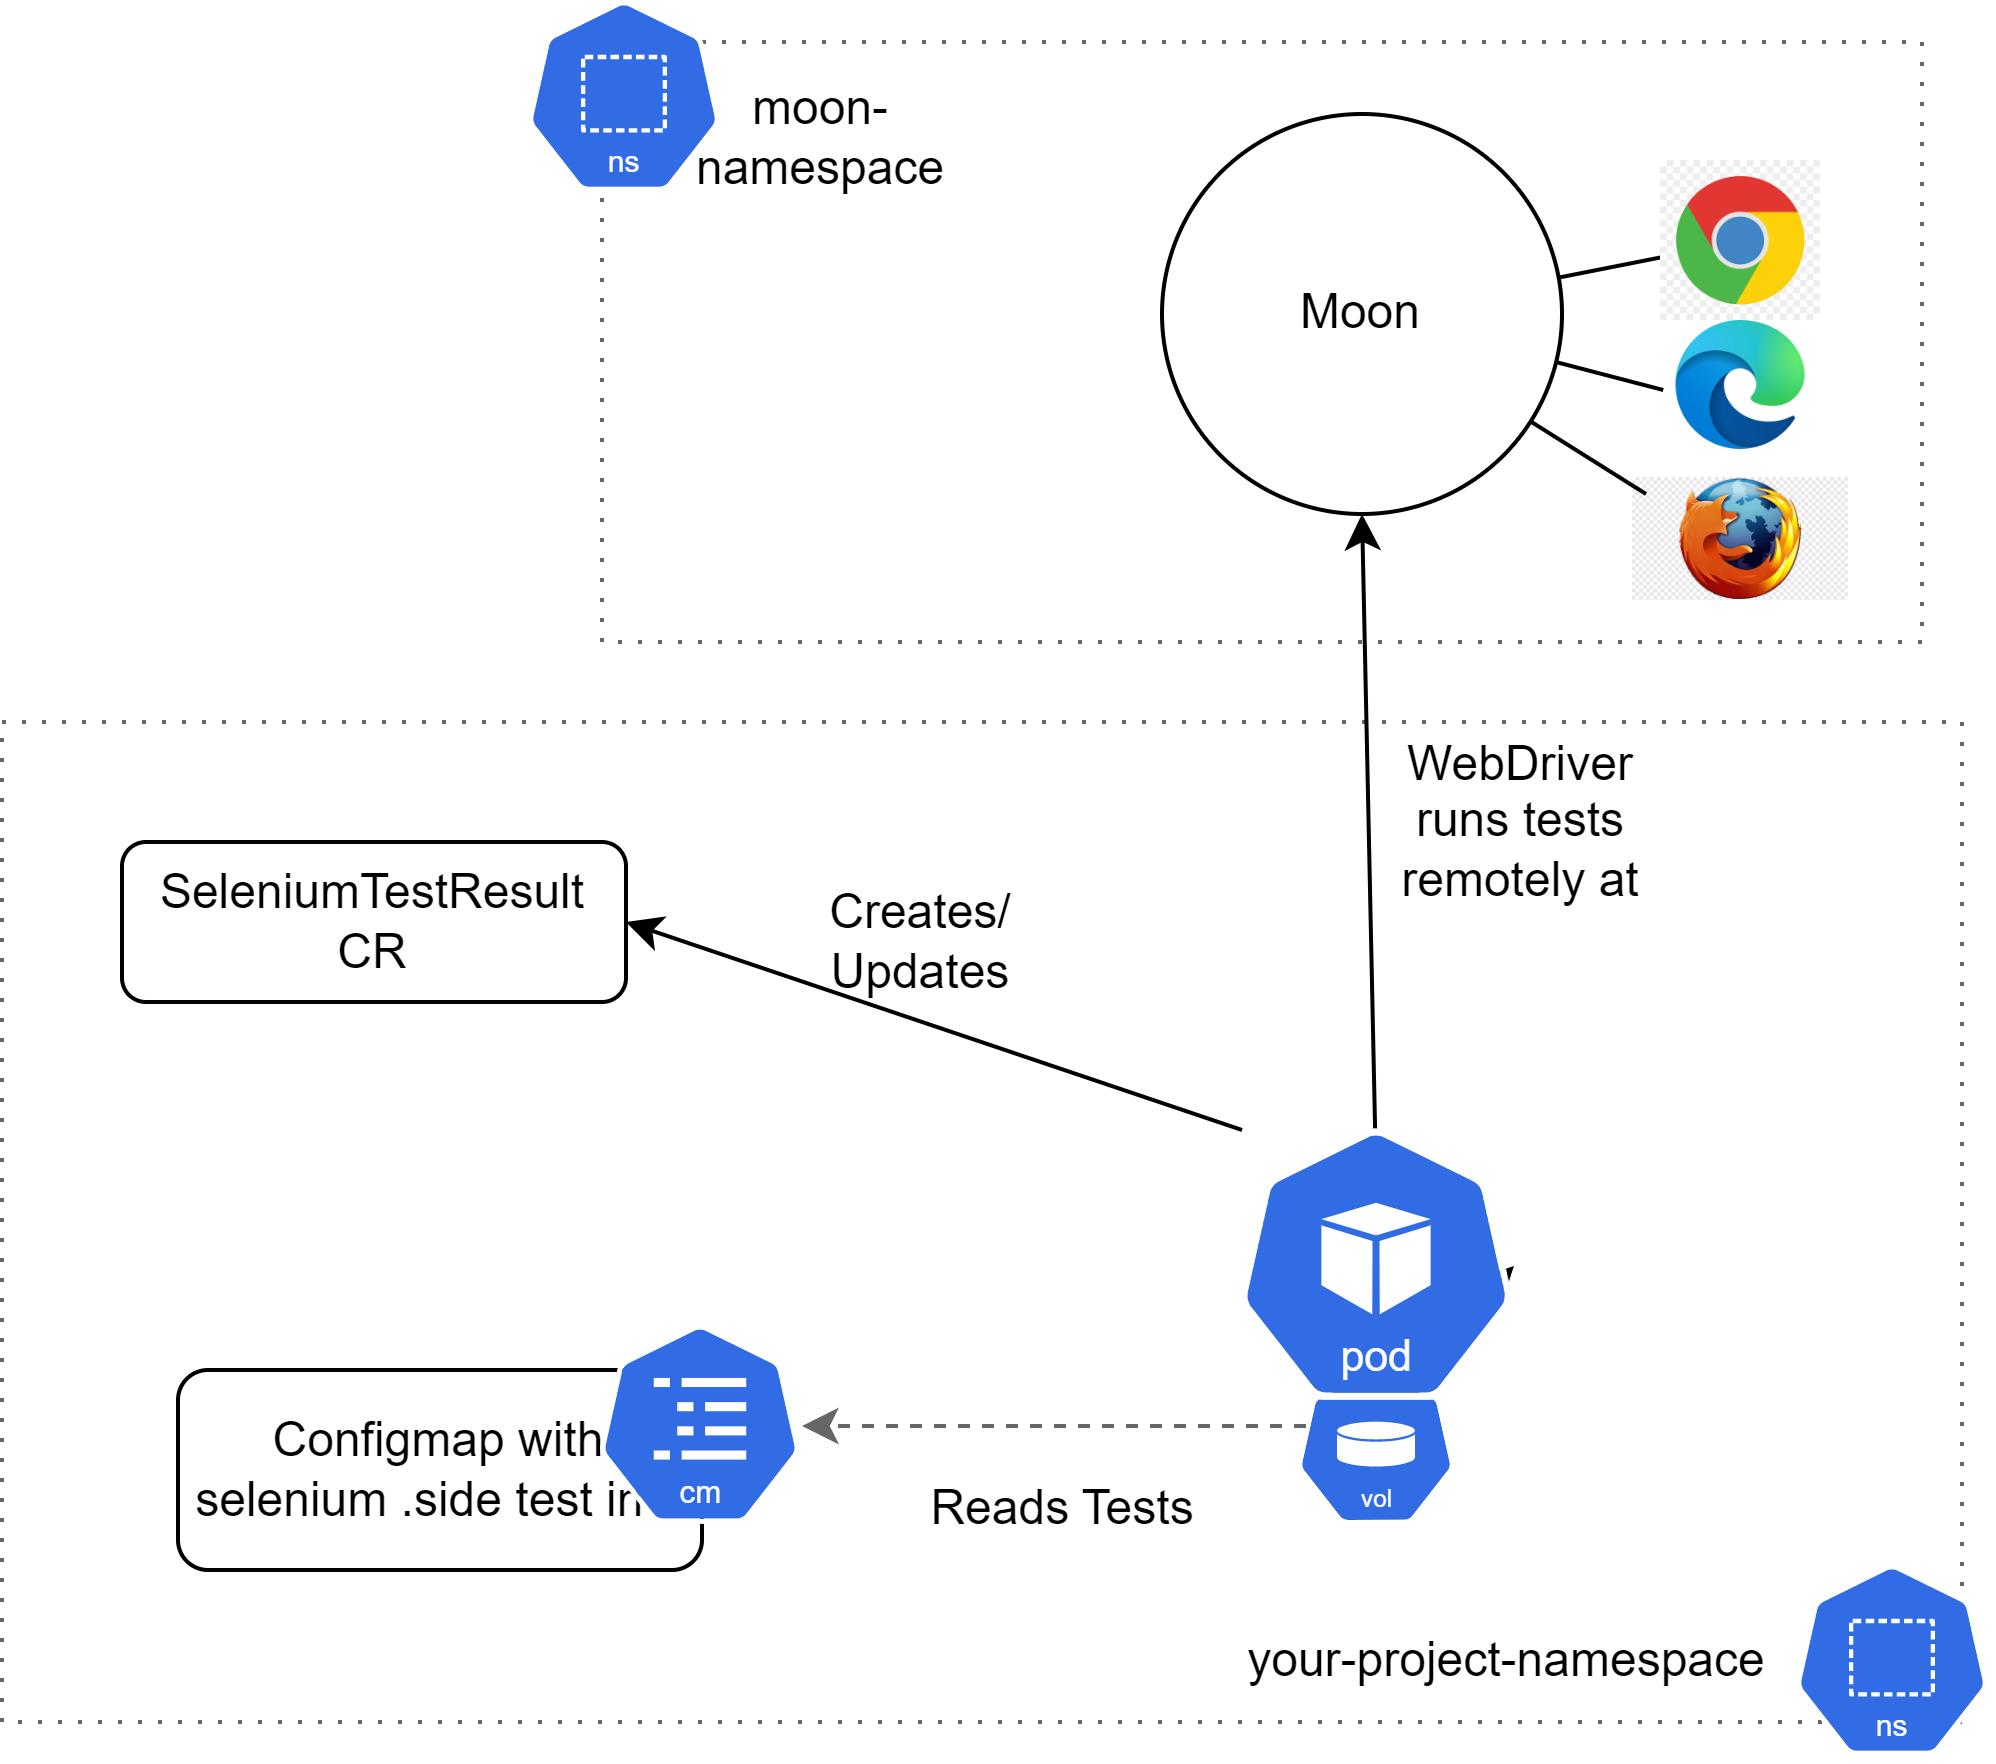
\includegraphics[width=1\textwidth]{selenium}
	\label{fig:selenium}
\end{figure}

\subsection{SeleniumTestResult CR and exposing results as Prometheus metrics}

A SeleniumTestResult custom resource corresponds to each test, and here is where the pod writes the results. In addition to the operator, its CRD is also deployed, and the operator has a go object, a controller, and a distinct reconcile method to handle it.

\begin{figure}[H]
	\centering
	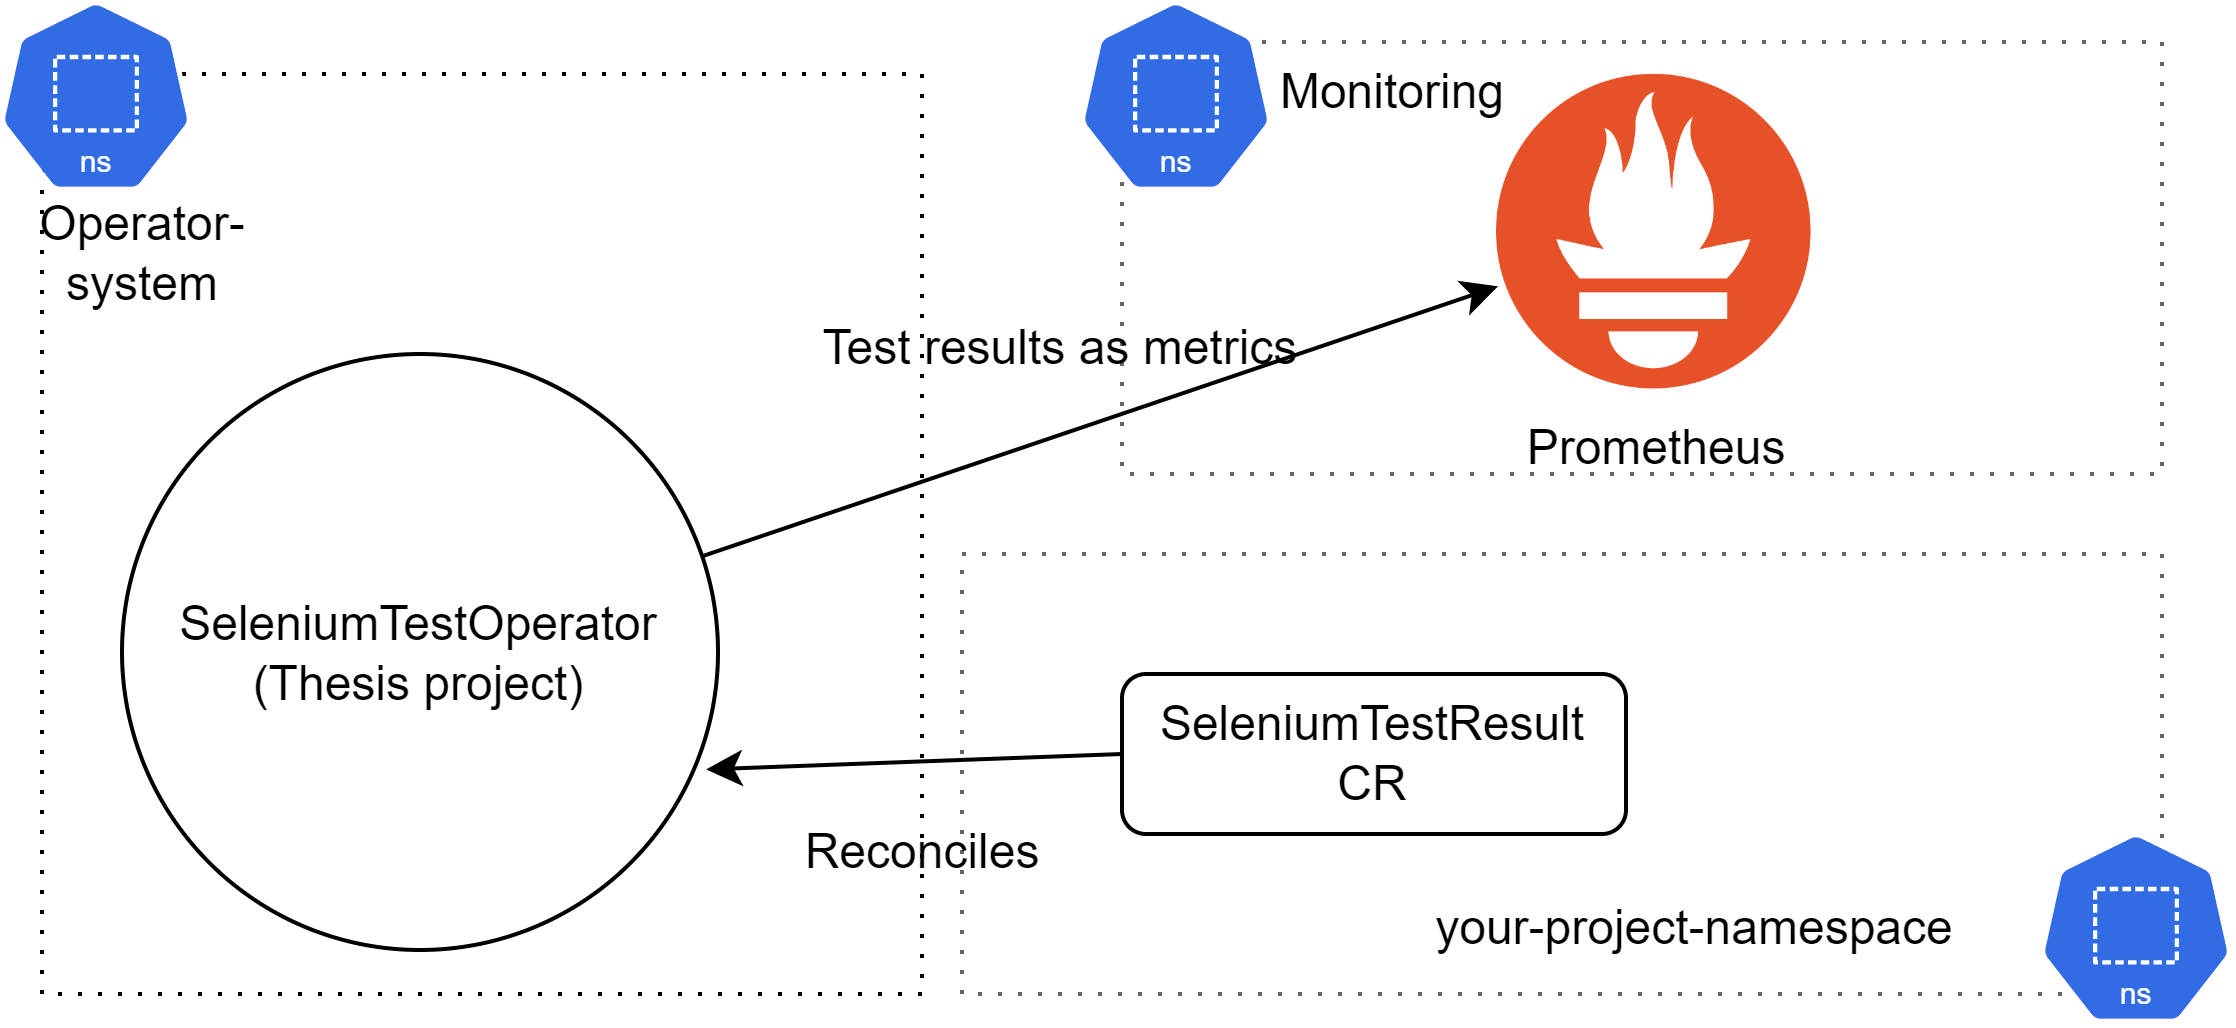
\includegraphics[width=1\textwidth]{prometheus}
	\label{fig:prometheus}
\end{figure}

The associated go object:
    
\begin{lstlisting}[language={Go}]
	// SeleniumTestResultSpec defines the desired state of SeleniumTestResult
	type SeleniumTestResultSpec struct {
		Success bool `json:"success"`
		EndTime int  `json:"endTime"`
	}
	type SeleniumTestResultStatus struct {}

	// SeleniumTestResult is the Schema for the seleniumtestresults API
	type SeleniumTestResult struct {
		metav1.TypeMeta   `json:",inline"`
		metav1.ObjectMeta `json:"metadata,omitempty"`

		Spec   SeleniumTestResultSpec   `json:"spec,omitempty"`
		Status SeleniumTestResultStatus `json:"status,omitempty"`
	}
\end{lstlisting}

Every time the SeleniumTestResult is modified, the reconcile function is called. The method uses Prometheus labels to expose the data, making it simple to sort the data for test results by name or namespace.

Metric declaration:

\begin{lstlisting}[language={Go}]
	var (
		test_results = prometheus.NewGaugeVec(
			prometheus.GaugeOpts{
				Name: "selenium_test_results",
				Help: "0 mean success, 1 means error",
			},
			[]string{"test_name", "namespace"},
		)
	)
	func init() {
		// Register custom metrics with the global prometheus registry
		metrics.Registry.MustRegister(test_results)
	}
\end{lstlisting}

For ease of reading in this documentation, logging and error handling are removed from the reconcile method demonstration below:

\begin{lstlisting}[language={Go}]
	func (r *SeleniumTestResultReconciler) Reconcile(ctx context.Context, req ctrl.Request) (ctrl.Result, error) {
		instance := &seleniumv1.SeleniumTestResult{}
		labels := prometheus.Labels{"test_name": instance.Name, "namespace": instance.Namespace}
		if instance.Spec.Success {
			test_results.With(labels).Set(1)
		} else {
			test_results.With(labels).Set(0)
		}
		return ctrl.Result{}, nil
	}
\end{lstlisting}

The metric viewed from a prometheus:

\begin{figure}[H]
	\centering
	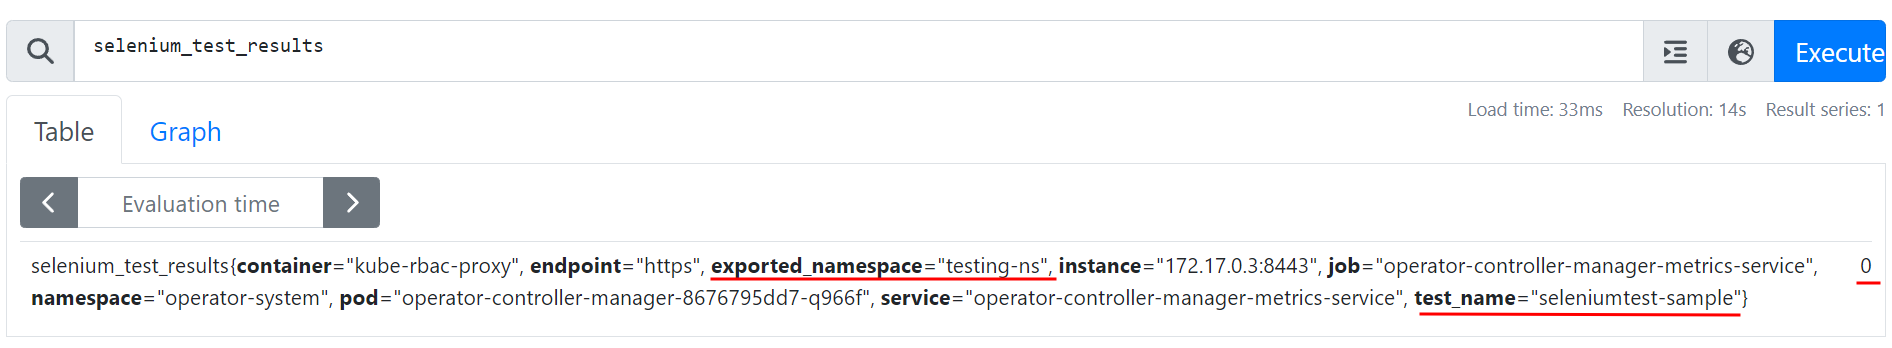
\includegraphics[width=1\textwidth]{prometheus_ui}
	\label{fig:prometheus_ui}
\end{figure}



\lstset{caption={Hello World in C++}, label=src:cpp}
\begin{lstlisting}[language={C++}]
#include <stdio>

int main() 
{
	int c;
	std::cout << "Hello World!" << std::endl;

	std::cout << "Press any key to exit." << std::endl;
	std::cin >> c;
	
	return 0;
}
\end{lstlisting}

\lstset{caption={Hello World in C\#}, label=src:csharp}
\begin{lstlisting}[language={[Sharp]C}]
using System;
namespace HelloWorld
{
	class Hello 
	{
		static void Main() 
		{
			Console.WriteLine("Hello World!");
			
			Console.WriteLine("Press any key to exit.");
			Console.ReadKey();
		}
	}
}
\end{lstlisting}

\section{Testiing}

A general Interval Branch and Bound algorithm is shown in Algorithm~\ref{alg:ibb}. An appropriate selection rule is applied in Step~\ref{step:selrule}.\\
Source of example: \href{https://www.inf.u-szeged.hu/actacybernetica/}{Acta Cybernetica (this is a hyperlink)}.

\begin{algorithm}[H]
\caption{A general interval B\&B algorithm} 
\label{alg:ibb} 
\textbf{\underline{Funct}} IBB($S,f$)
\begin{algorithmic}[1] % display line numbers before every n line, here n = 1
\State Set the working list ${\cal L}_W$ := $\{S\}$ and the final list ${\cal L}_Q$ := $\{\}$     
\While{( ${\cal L}_W \neq \emptyset$ )} \label{alg:igoend}
	\State  Select an interval $X$ from ${\cal L}_W$ \label{step:selrule}\Comment{Selection rule}  
	\State Compute $lbf(X)$ \Comment{Bounding rule}		  
	\If{$X$ cannot be eliminated} \Comment{Elimination rule}
		\State Divide $X$ into $X^j,\ j=1,\dots, p$, subintervals   \Comment{Division rule}
		\For{$j=1,\ldots,p$}
			\If{$X^j$ satisfies the termination criterion} \Comment{Termination rule}
				\State Store $X^j$ in ${\cal L}_W$ 
			\Else
				\State Store $X^j$ in ${\cal L}_W$ 
			\EndIf
		\EndFor  
	\EndIf
\EndWhile
\State \textbf{return} ${\cal L}_Q$
\end{algorithmic}
\end{algorithm}
